The XML benchmarking project XMARK~\citep{xmark/original} is one of the most popular and commonly used XML benchmarking project to date. It provides a small executable tool called \textit{xmlgen} that allows to create a synthetic XML dataset based on a fixed schema describing an Internet auctions database. The xmlgen can be used to build  a single record with a large, hierarchical XML tree structure. A factor is specified to scale the generated data, ranging from a few kilobytes to any arbitrary size limited by the capacity of the system. The textual part of resulting XML document is constructed from 17,000 most frequently occurring words of Shakespeare's plays.

\subsection{Dataset}\label{xmark-dataset}
The main entities of XMark data are in two groups.First group consists of  \textit{person}, \textit{open\_auction}, \textit{closed\_auction}, \textit{item} and \textit{category}. The second group entities \textit{annotation} and \textit{description} are natural language text and document-centric element structure. The relationship between the entities in group one are expressed in reference and the second group entities are embedded into subtree of first group entities. Figure~\ref{fig:xmark-tree} shows XMark dataset with following properties:
\label{xmark:desc:each}
\begin{itemize}	
	\item
		\textit{people} are collection of \textit{person} that are connected to buyer and seller of open\_auctions, closed\_auctions, etc. Each person has an unique identifier \textit{id} to reference to another entities like open\_auctions and closed\_auctions.
	\item
		\textit{items} are objects for sale or already sold. Each \textit{item} carries a unique identifier \textit{id} and has properties like name, payment information, description and a reference to the seller that are encoded as elements. Each item belongs to the world's regions \texttt{africa}, \texttt{asia}, \texttt{australia}, \texttt{europe}, \texttt{namerica} and \texttt{samerica} as a parent of an item element.
	\item
		\textit{open\_auctions} referred to current auctions that contain bid history(increase/decrease over time) with reference to bidder and seller reference, current bid, the time interval of bid accepted, the status of the transaction, a reference to the item being sold etc.
	\item
		\textit{closed\_auctions} contain auctions that are successfully completed bidding. They have properties like buyer and seller information reference to \textit{person}, a reference to an sold items ,amount of price, quantity of sold items, date of transaction, type of transaction and many more.
	\item 
		\textit{categories} are used to classify the items. Each category has an unique identifier that is used to reference in item, a name and a description.
	\item
		  A \texttt{catgraph} links categories into a network.  The full semantics of XMark dataset can be found in~\cite{xmark/original}.
\end{itemize}
The full ER-Diagram of XMark dataset is illustrated in Fig.~\ref{fig:xmark-schema}. 
\begin{figure}[H]
	\centering
	\subfloat[Reference in \textit{XMark}]{
		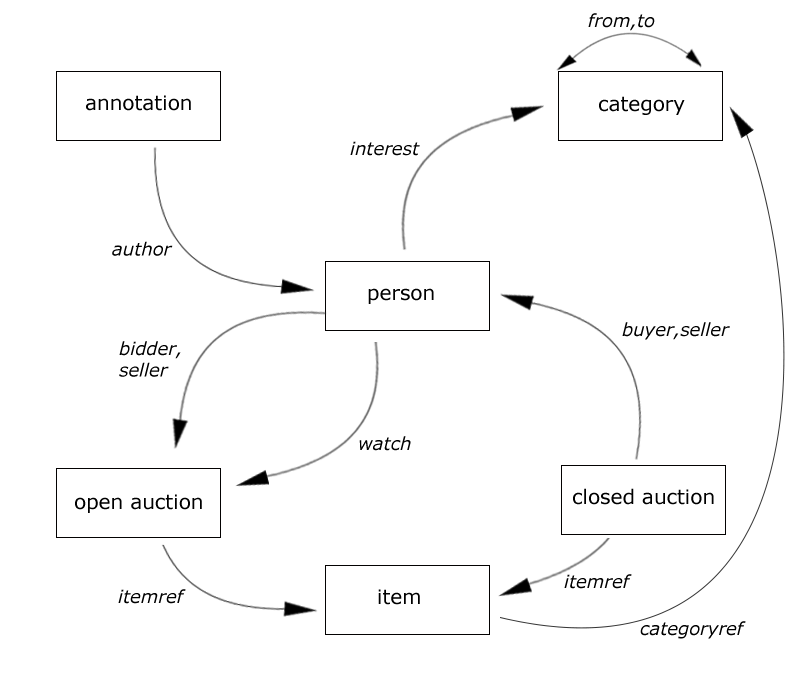
\includegraphics[width=0.40\textwidth]{img/xmark/101}{ %xmark-references.png
			\label{fig:xmark-reference}
		}
	}
	\centering
	\subfloat[Reference in \textit{XMark} dataset tree]{
		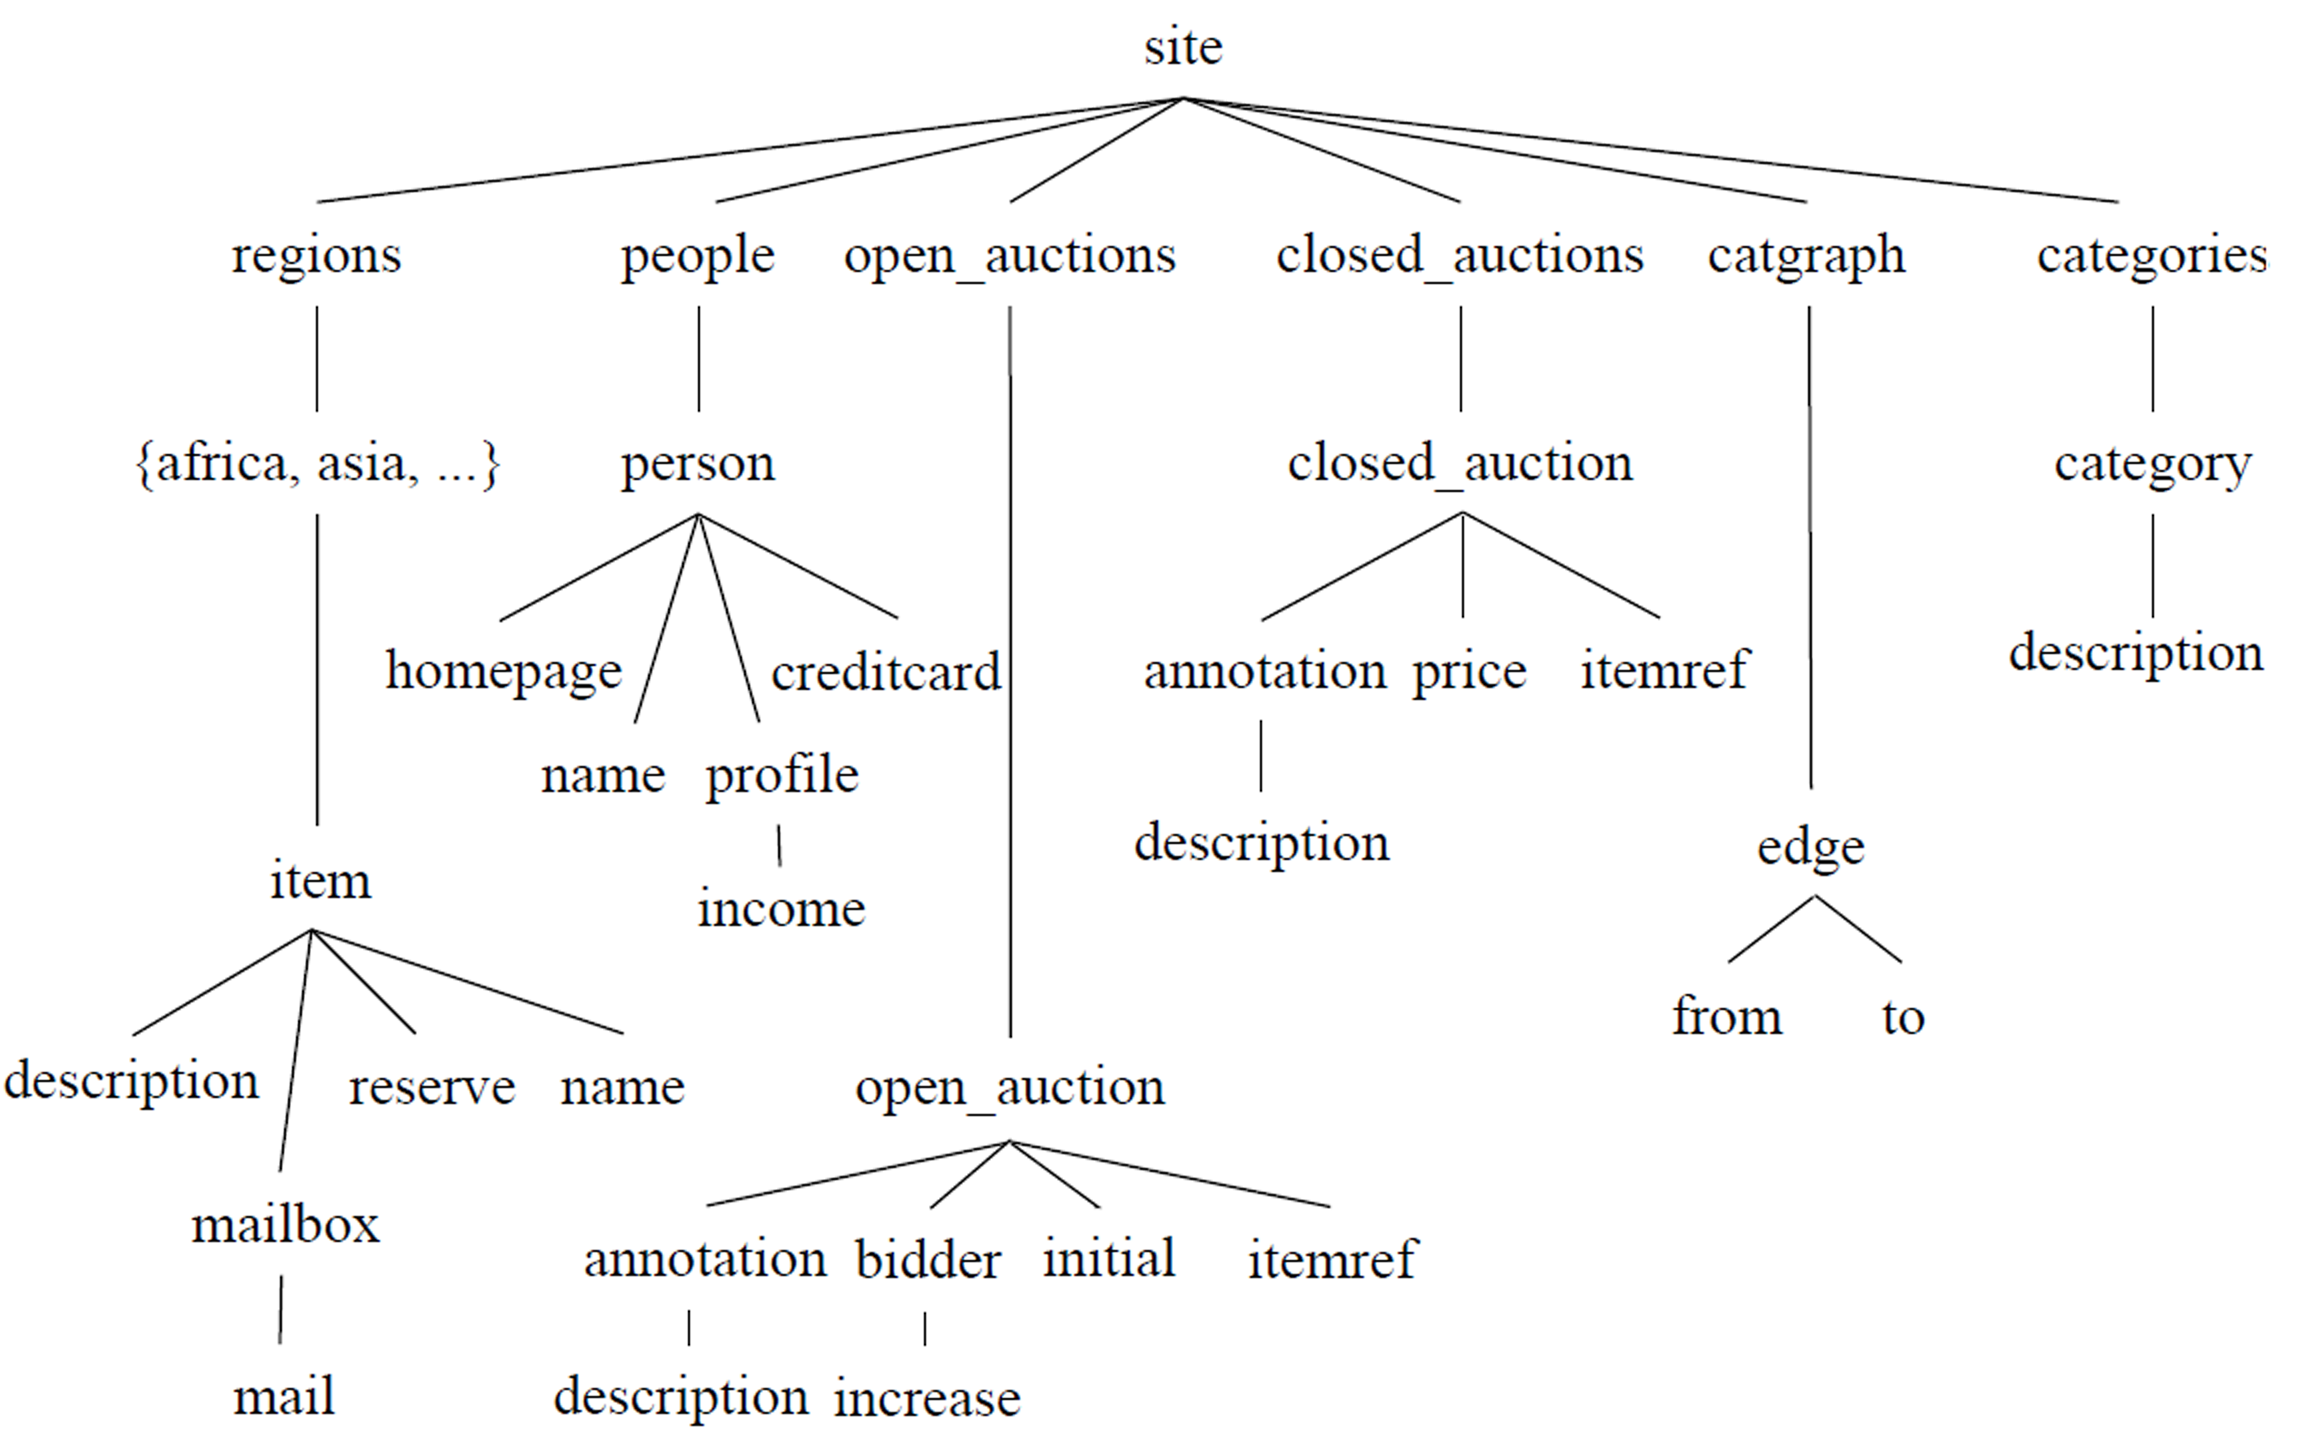
\includegraphics[width=0.4\textwidth]{img/xmark-tree.png}{
			\label{fig:xmark-tree}
		}
	}
	\caption{XMark data tree and reference~\citep{xmark/original}}
	\label{fig:xmark-tree-reference}
\end{figure}
\begin{figure}[H]
	\centering
	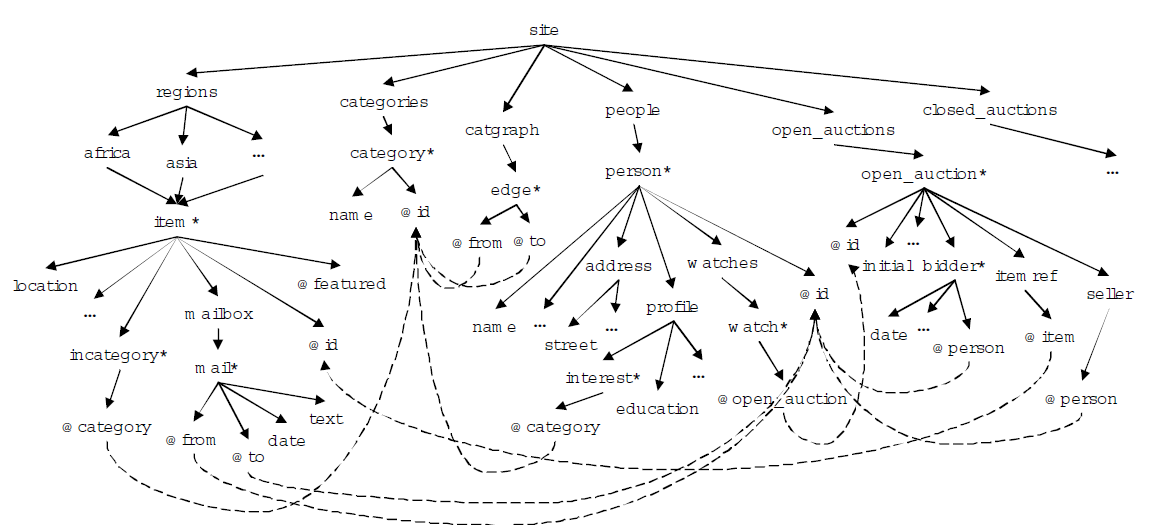
\includegraphics[width=0.90\textwidth]{img/xmark-schema-4}
	\caption{XMark ER-Diagram. Nodes, solid arrows, and dashed arrows represent schema elements (or attributes, with prefix '@'), structural links, and value links, respectively. Elements with suffix '*' are of SetOf type\citep{xmark/schema-sumerize}}
	\label{fig:xmark-schema}
\end{figure}

\label{xmark-queries}
\subsection{XMark Queries}
The XMark project contains XQuery queries that focuses on various aspect of language such as aggression, reference, ordering, wildcard expressions, joins, user defined functions, etc.\citep{xmark/mlynkova2008xml}.The textual representation of 20 different XQuery are reprinted in  Table~\ref{tab:xmark-queries}. These queries are divided into different categories  based on the  multiple functionalities of XQuery: 
\begin{enumerate}[label=\arabic*.]
\item  First category tests execution of exact match of string in specified path and consists of only query Q1.
\item It  helps to analyze order access of an XML document. Query Q2, Q3 and Q4 are grouped here.
\item  Query Q5 is evaluates the casting of a value.
\item Queries Q6 and Q7  evaluate regular path expressions.

\item This category investigates the referencing of a document to another and consists of query Q8 and Q9

\item Query Q10 reconstructs a complex results from the result of a query

\item Two queries, Q11 and Q12 are join query based on values.  The difference between this category's queries and reference queries Q8 and Q9 is that references are specified in DTD and may optimize with object identifiers whereas Q11 and Q12 are have join on the basis of values.

\item Query Q13  benchmarks the portion reconstruction of original XML document.

\item In this category the full text search  using single word is implemented. Q14 is in this category

\item The purpose of queries 15 and 16 is to observe the path traversals without using wildcards.

\item Query Q17 tests the ability to deal with missing values

\item This category deals with user defined functions and contains query Q18

\item The query Q19 is use to evaluate Sorting.

\item The last category observe the aggregation with the help of query 20.

\end{enumerate}

\begin {table}[htpb] 
\centering
\caption {The XMark queries. Source:\citep{xmark/original}}
\label {tab:xmark-queries}
\begin{tabular}{r|l}
	\hline
	Q1&Return the name of the person with ID 'person0'.\\
	\hline
	Q2&Return the initial increase of all open auctions.\\
	\hline
	Q3&Return the first and current increase of all open auctions whose current\\
	&increase is at least twice as high as the initial increase.\\
	\hline
	Q4&List the reserves of those open auctions where a certain person issued\\
	&a bid before another person.\\
	\hline
	Q5&How many sold items cost more than 40.\\
	\hline
	Q6&How many items are listed on all continents?\\
	\hline
	Q7&How many pieces of prose are in our database?\\
	\hline
	Q8&List the names of persons and the number of items they bought.\\
	&(Joins person, closed\_auction)\\
	\hline
	Q9&List the names of persons and the names of items they bought in Europe.\\
	&(Joins person\_auction, item)\\
	\hline
	Q10&List all persons according to their interest; use French markup\\
	&in the result.\\
	\hline
	Q11&For each person, list the number of items currently on sale whose\\
	&price does not exceed 0.02\% of the person's income.\\
	\hline
	Q12&For each richer-than-average person, list the number of items currently\\
	&on sale whose price does not exceed 0.02\% of the person's income.\\
	\hline
	Q13&List the names of items registered in Australia along with\\
	&their description.\\
	\hline
	Q14&Return the names of all items whose description contains the word 'gold'.\\
	\hline
	Q15&Print the keywords in emphasis in annotations of closed auctions.\\
	\hline
	Q16&Return the IDs of those auctions that have one or more keywords\\
	&in emphasis.\\
	\hline
	Q17&Which persons don't have a homepage?\\
	\hline
	Q18&Convert the currency of the reserve of all open auctions to\\
	&another currency.\\
	\hline
	Q19&Give an alphabetically ordered list of all items along with their location.\\
	\hline
	Q20&Group customers by their income and output the cardinality of each\\
	&group.\\
	\hline
\end{tabular}
\end {table}
